\documentclass[12pt]{article}
\usepackage[utf8]{inputenc}
\usepackage[]{multicol}
\usepackage[auth-lg]{authblk}
\usepackage[margin=1.4in]{geometry}
\usepackage[]{graphicx}
\usepackage[]{ctable}

\title{Dynamic Programming in RNA Folding Software and Improvements to the Current Regime}

\begin{document}
\author{Jianglin Liu}
\author{Bingxi Li}
\author{Gregory Rehm}
\affil{\normalsize{University of California, Davis}
\{\texttt{jiliu, bxli, grehm\}@ucdavis.edu}}
\maketitle

\begin{abstract}
Finding the secondary structure of RNA is important for understanding how RNA will interact in a cell. Frequently computational algorithms are used to determine structure due to difficulties extracting good \textit{in vivo} data of RNA structures. Many of the algorithms for RNA folding are computationally complex. In this paper we establish benchmarks for two commonly used RNA folding packages, mfold, and RNAFold Vienna, and compare them to an improved Four-Russians folding algorithm. We show ... These results will help software maintainers to understand the benefit of updating their algorithms. The results will also help guide users when choosing RNA folding software when looking for the most computationally optimal package.
\end{abstract}
\section{Introduction}
\par RNA is an essential macromolecule used in protein formation and performs other essential functions within the body\cite{turner}. RNA does not stay in single stranded form and instead folds on itself to create the lowest energy conformation possible to ensure thermodynamic stability\cite{herschlag}. When folding, RNA forms a 2D secondary structure\cite{mccaskill} with A matching to U and G to C (figure 1).  Using this data we can find a 3D tertiary structure\cite{mccaskill}.
\begin{figure}[h!]
  \centering
  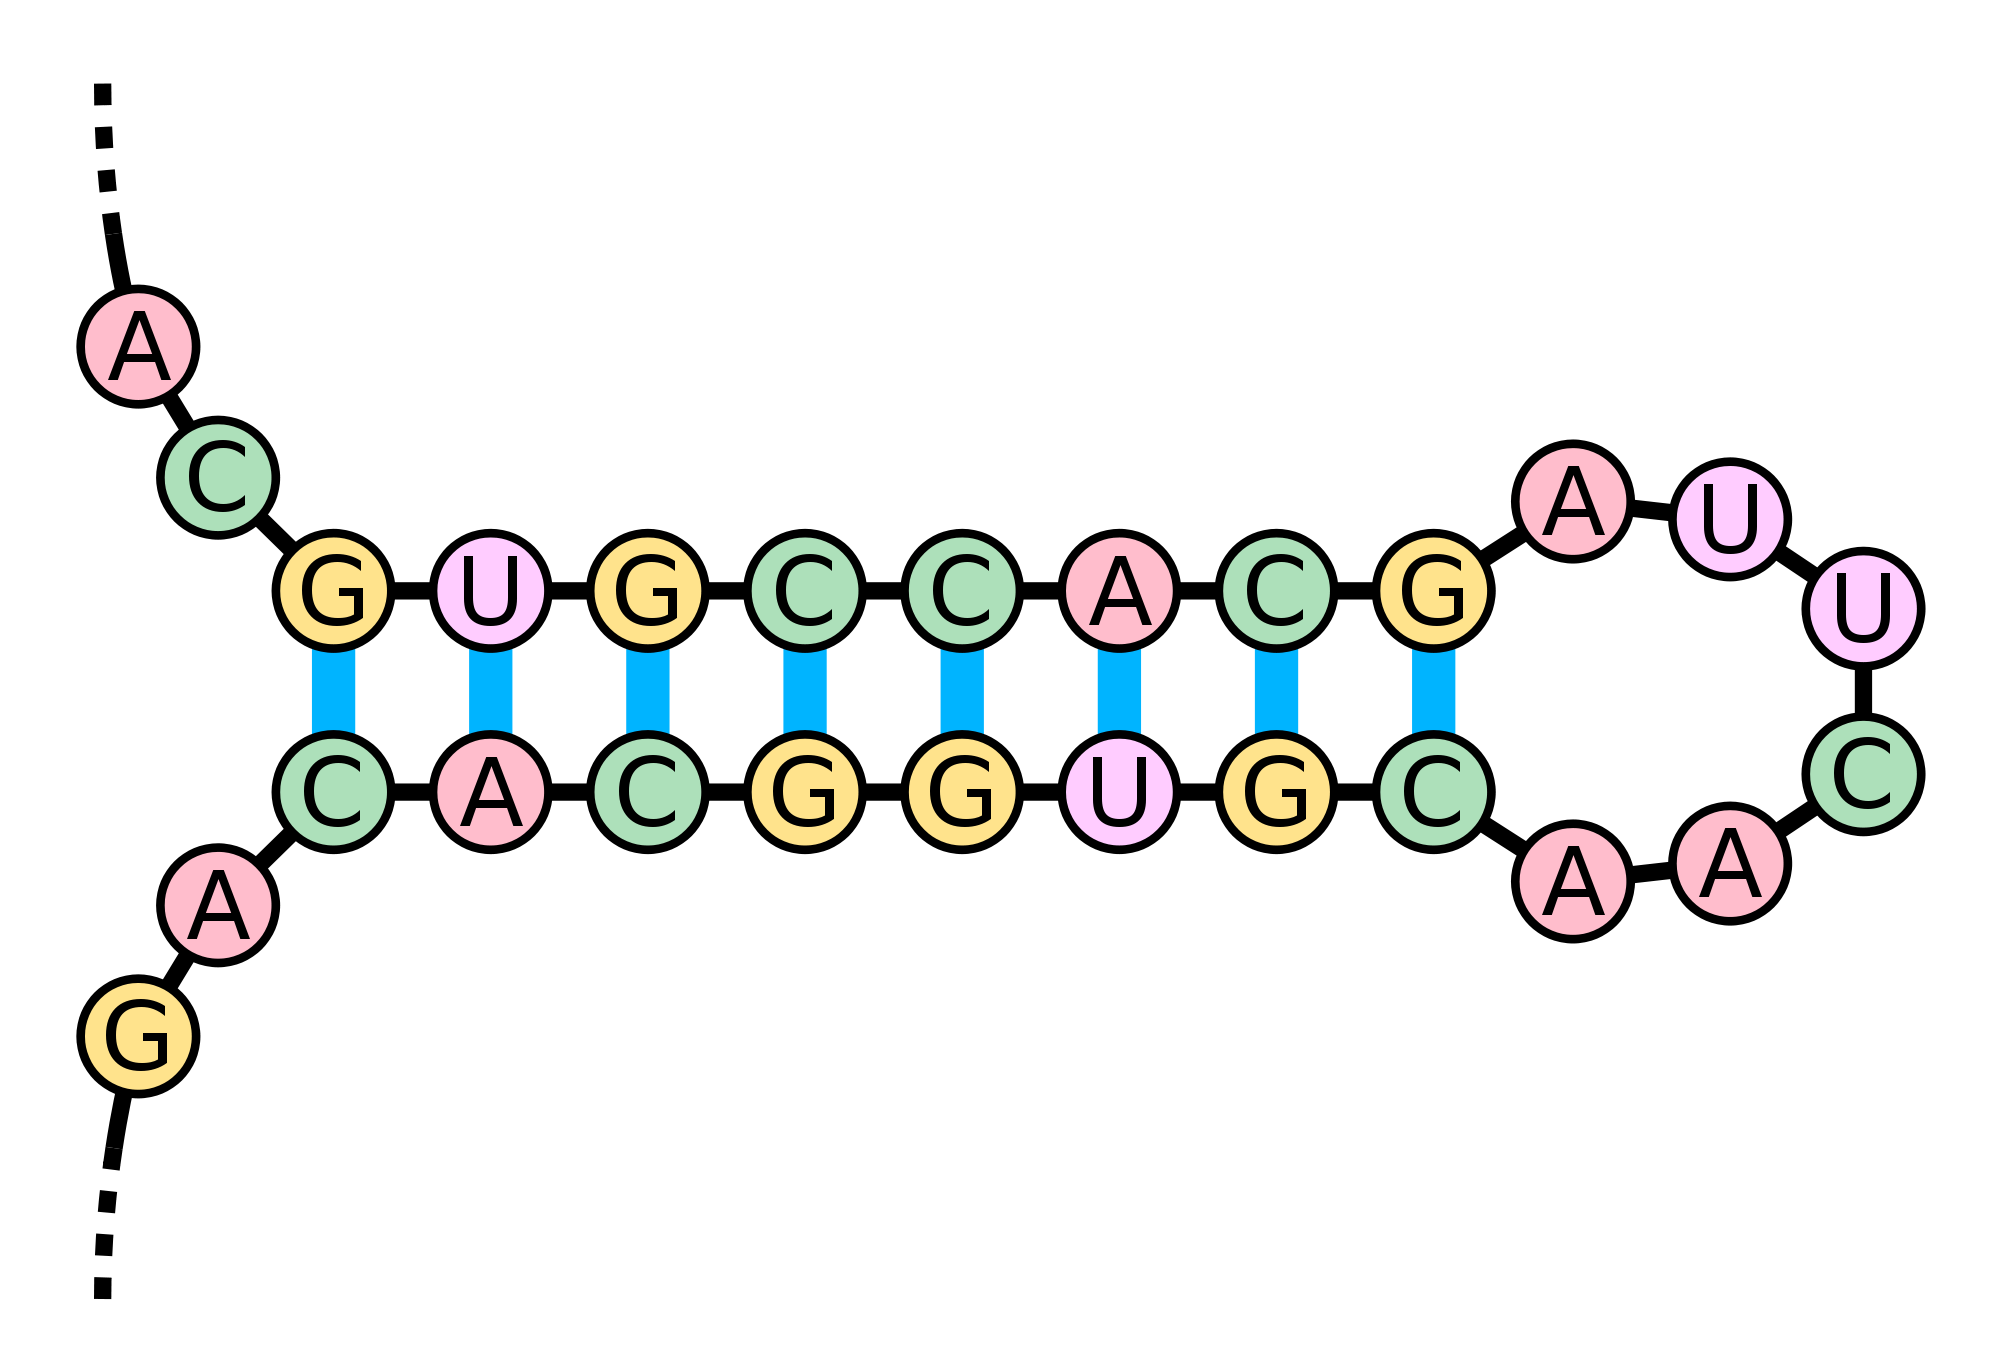
\includegraphics[keepaspectratio, scale=0.12]{fold-example.png}
  \caption{Example of an RNA molecule folding}
  \label{fig:RNA Folding}
\end{figure}
\par Our paper focuses on benchmarking 2D secondary structure prediction software based off the Nussinov dynamic programming algorithm\cite{nussinov} for RNA folding. This algorithm is $O(n^3)$ time complexity. There have been multiple attempts to parallelize the Nussinov algorithm[!CITE!] which have resulted in large speed increases, however, CPU intensive algorithms only slightly lowered the bound up until 2011[!CITE!]. In 2011 the Nussinov bound that was improved by the Frid-Gusfield Four Russians method which established you could perform the DP method in $O(\frac{n^3}{log(n)})$ time\cite{gusfield}. Later a parallel method of the Four Russians algorithm presented proof that you can lower this bound to $O(\frac{n^2}{log(n)})$ inside an NVIDIA CUDA environment\cite{balaji}.
\par There are two major RNA folding software packages, mfold\cite{zuker1989,zuker1981}, and the Vienna RNA Package\cite{vienna}. These both utilize the Nussimov method to return results of the RNA secondary structure by finding the lowest possible thermodynamic conformations of the RNA\cite{zuker1981,vienna}. In order to tell which was faster we performed application level benchmarks\cite{eulogy} to see which of these two applications could more quickly fold arbitrary length RNA of the circular and linear variety. We then performed micro-benchmarks\cite{sysperformance} of the folding algorithms utilized in mfold and Vienna for both circular and linear RNA, and then compared that to equivalent benchmarks for the Four Russians and parallel Four Russians algorithms. The first thing we found when comparing mfold and Vienna was ... . When we compared mfold and Vienna to the Four Russians algorithms we found that without a graphics card and parallel processing capabilities a machine can see speed ups of ... in mfold and ... in Vienna for linear RNA. For circular RNA speed increases change to ... in mfold and ... in Vienna. With a graphics card and parallel processing folding clusters can see increases of up to ... for mfold and ... in Vienna. Circular RNA also sees speed bumps of ... in mfold and ... in Vienna.
\par These results show us that ... for natively differentiating between mfold and Vienna. They also help explain that both pieces of software can experience significant speed increases if they implemented the Frid-Gusfield method. Furthermore the authors of this paper would recommend both software packages to support GPU hardware to achieve even greater speed gains when inside a parallel capable environment.

\section{Methods}
Benchmarking is renown as a difficult thing to perform effectively\cite{sysperformance,eulogy}. There are so many things that can be going on in a computer at any one moment that it is completely possible that a benchmark can give inaccurate information due to a conflicting process running on the computer\cite{sysperformance}. As a result we used a machine solely dedicated for benchmarking and no other tasks. We also standardized on the following specifications for our runs:
\begin{center}
    \begin{tabular}{ccc}
        \specialrule{.1em}{.05em}{.05em}
        \textbf{Architecture} & \textbf{Operating System} & \textbf{Compiler} \\ \hline
        blah & Linux & GCC xx \\ \hline
        " & " & Fortran 77 \\ \hline
        " & " & python3 \\ \hline
        " & " & NVIDIA CUDA \\
        \specialrule{.1em}{.05em}{.05em}
    \end{tabular}
\end{center}
We used the following applications with corresponding versions and requirements in our test runs:
\begin{center}
    \begin{tabular}{ccc}
        \specialrule{.1em}{.05em}{.05em}
        \textbf{Application} & \textbf{Version} & \textbf{Requirements} \\ \hline
        mfold & 3.6 & GCC, Fortran \\ \hline
        RNAfold Vienna  & xxx & GCC \\ \hline
        Frid-Gusfield Four Russians & N/A & python3 ?? \\ \hline
        Parallel Four Russians & N/A & GCC, NVIDIA CUDA \\
        \specialrule{.1em}{.05em}{.05em}
    \end{tabular}
\end{center}
Our testing architecture was laid out where we would SSH into the benchmarking machine and then execute tests. Test results would then be reported back to the user's central machine where they could be stored in a database for later analysis (figure 2). Our testing required no internet connectivity besides the ssh access required to initiate our testing so all calculations were performed locally. Furthermore there were few I/O read/writes required as we will show so there is very little chance that I/O was a factor on our results.
\begin{figure}[h!]
  \centering
  \includegraphics[keepaspectratio, scale=0.7]{benchmarking-architecture.png}
  \caption{Test Architecture}
  \label{fig:Testing Arch}
\end{figure}

\subsection{Micro-benchmarks}
The easiest type of benchmark to perform is the micro-benchmark. The micro-benchmark is a single piece of code executed many times in serial so that we can get a good profile of its run characteristics. Once these characteristics are observed we can then make inferences about its performance and ways that it can be improved. Micro-benchmarks have the downside of losing generality of performance across the entire application\cite{eulogy}. A good example of this is if an IO heavy function made many consecutive calls to the \textit{read} function on the OS while the rest of the application made no calls to \textit{read} whatsoever. So if we tried to generalize this one function to the rest of the application we would misguidedly attempt to optimize disk IO across our entire system.
\par We avoid this trap in our paper by benchmarking only parts of the code that execute the Nussinov algorithm in mfold and the Vienna package. We then
\subsection{Application Benchmarks}
One type of benchmark we can perform is an application level benchmark. Applications generally are composed of many different modules an processes and sometime

\par Micro-benchmarking is the process of running small pieces of code and then testing the amount of time it takes to execute. These tests are performed many times to return some kind of statistical distribution of run times and other relevant information.
\section{Results}

\section{Discussion}
\begin{thebibliography}{56}
\bibitem{gusfield}
Frid Y, Gusfield D.
\textit{A simple, practical and complete O($n^3$)-time
algorithm for RNA folding using the Four-Russians Speedup}.
Algorithms Mol Biol 2010, 5:13
\bibitem{balaji}
Venkatachalam B, Gusfield D.
\textit{Faster algorithms for RNA-folding using the Four-Russians method}.
Algorithms for Molecular Biology20149:5.
\bibitem{nussinov}
Nussinov R, Jacobson A.
\textit{Fast algorithm for predicting the secondary structure of
single-stranded RNA}.
Proc. Nati. Acad. Sci. USA Vol. 77, No. 11, pp. 6309-6313, November 1980.
\bibitem{turner}
Mathews D, Turner D.
\textit{Prediction of RNA secondary structure by free energy
minimization}.
Current Opinion in Structural Biology 2006, 16:270–278.
\bibitem{mccaskill}
McCaskill J.S.
\textit{The Equilibrium Partition Function and Base Pair
Binding Probabilities for RNA Secondary Structure.}
Biopolymers, Vol. 29,1105-1119 (1990)
\bibitem{herschlag}
Herschlag D.
\textit{RNA Chaperones and the RNA Folding Problem}.
Vol. 270, No. 36, Issue of September 8, pp. 20871–20874, 1995
\bibitem{vienna}
Hofacker I. L, Fontana W, Stadler P. F, Bonhoeffer L. S, Tacker M, Schuster P.
\textit{Fast Folding and Comparison of RNA Secondary Structures}.
Monatshefte ftir Chemie 125, 167-188 (1994)
\bibitem{zuker1989}
Zuker M.
\textit{Computer Prediction of RNA Structure}.
Methods in Enzymology, vol. 180.
\bibitem{zuker1981}
Zuker M, Steigler P.
\textit{Optimal computer folding of large RNA sequences using thermodynamics and auxiliary information}.
Nucleic Acids Research vol. 9 Number 11981.
\bibitem{sysperformance}
Gregg B.
\textit{Systems Performance; Enterprise and the Cloud}.
Pearson Education 2014 Upper Saddle River, NJ
\bibitem{eulogy}
Cantrill B.
\textit{Eulogy for a benchmark}.
http://dtrace.org/blogs/bmc/2009/02/02/eulogy-for-a-benchmark/.
2009.
\end{thebibliography}

\end{document}
